\subsection{Heater Design}
TiN microheaters are placed \SI{1}{\micro\meter} above the waveguide
core and extend along the full coupling-section length $L_c$.  A
resistance of approximately \SI{1}{\kilo\ohm} per heater is targeted to
allow direct CMOS-compatible driving voltages ($\leq \SI{3.3}{\volt}$).

\subsection{Tuning Efficiency}
The thermal tuning efficiency is defined as
\begin{equation}
  \eta_\text{th} = \frac{d\lambda_\text{res}}{dP_\text{heater}}
                 = \frac{\lambda_\text{res}}{n_g}\,\Gamma\,
                   \frac{dn}{dT}\,\frac{\partial T}{\partial P},
  \label{eq:tuning_efficiency}
\end{equation}
where $\partial T / \partial P$ is the heater thermal resistance
(\SI{}{\kelvin\per\milli\watt}).  Finite-element thermal simulation
(COMSOL, 2-D) yields $\partial T / \partial P = \SI{11.2}{\kelvin\per\milli\watt}$,
resulting in a tuning efficiency of \SI{688}{\pico\meter\per\milli\watt}.

\subsection{Tuning Range and Power Budget}
A full ITU channel grid shift of $\Delta\lambda = \SI{0.8}{\nano\meter}$
requires a heater power of approximately \SI{1.2}{\milli\watt}.  To
cover a $\pm\SI{2}{\nano\meter}$ range (for post-fabrication correction
of process variations), a maximum power of $\sim\SI{3}{\milli\watt}$
per channel is needed.

\begin{figure}[!t]
  \centering
  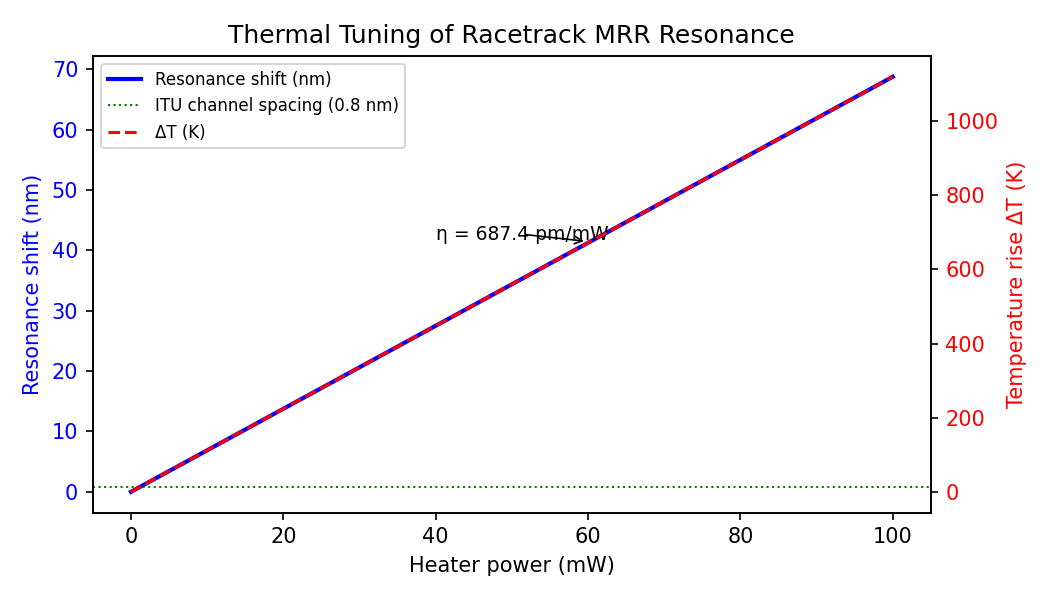
\includegraphics[width=\columnwidth]{figures/thermal_tuning}
  \caption{Resonance wavelength shift as a function of heater power.
           Circles: analytical model data points; solid line: linear fit
           with slope \SI{688}{\pico\meter\per\milli\watt}.}
  \label{fig:thermal}
\end{figure}

\subsection{Thermal Crosstalk}
Thermal crosstalk between adjacent channels is estimated from the 2-D
heat-diffusion model.  With a channel pitch of \SI{100}{\micro\meter},
the temperature rise on an adjacent ring due to activation of a
neighbouring heater is $<\SI{0.5}{\kelvin}$, producing a parasitic
resonance shift of $<\SI{10}{\pico\meter}$---well below the channel
spacing.
